% Multistate Markov diagram for literacy transitions
% Generated from R analysis
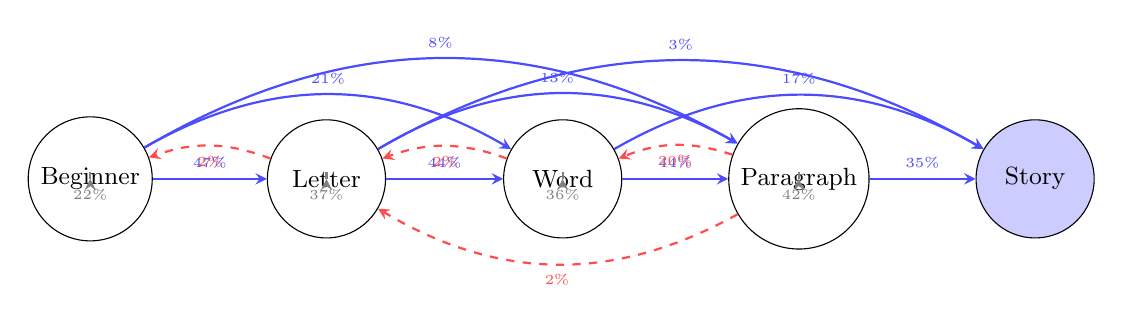
\begin{tikzpicture}[
  state/.style={circle, draw, minimum size=1.5cm, font=\small},
  forward/.style={->, >=stealth, thick, blue!70},
  backward/.style={->, >=stealth, thick, red!70, dashed},
  stay/.style={->, >=stealth, thick, gray},
]

% States
\node[state] (beg) at (0,0) {Beginner};
\node[state] (let) at (3,0) {Letter};
\node[state] (wrd) at (6,0) {Word};
\node[state] (par) at (9,0) {Paragraph};
\node[state, fill=blue!20] (sto) at (12,0) {Story};

% Transitions
\draw[stay] (beg) to node[below, font=\tiny] {22\%} (beg);
\draw[forward] (beg) to node[above, font=\tiny] {47\%} (let);
\draw[forward, bend left=30] (beg) to node[above, font=\tiny] {21\%} (wrd);
\draw[forward, bend left=30] (beg) to node[above, font=\tiny] {8\%} (par);
\draw[backward, bend right=20] (let) to node[below, font=\tiny] {2\%} (beg);
\draw[stay] (let) to node[below, font=\tiny] {37\%} (let);
\draw[forward] (let) to node[above, font=\tiny] {44\%} (wrd);
\draw[forward, bend left=30] (let) to node[above, font=\tiny] {13\%} (par);
\draw[forward, bend left=30] (let) to node[above, font=\tiny] {3\%} (sto);
\draw[backward, bend right=20] (wrd) to node[below, font=\tiny] {2\%} (let);
\draw[stay] (wrd) to node[below, font=\tiny] {36\%} (wrd);
\draw[forward] (wrd) to node[above, font=\tiny] {44\%} (par);
\draw[forward, bend left=30] (wrd) to node[above, font=\tiny] {17\%} (sto);
\draw[backward, bend left=30] (par) to node[below, font=\tiny] {2\%} (let);
\draw[backward, bend right=20] (par) to node[below, font=\tiny] {20\%} (wrd);
\draw[stay] (par) to node[below, font=\tiny] {42\%} (par);
\draw[forward] (par) to node[above, font=\tiny] {35\%} (sto);

\end{tikzpicture}
